% Kapitel 1 - Einleitung
\section{Einleitung}

In diesem Kapitel wird zunächst die Motivation für dieser Arbeit dargelegt. Danach wird auch auf die Zielsetzung eingegangen, die das Thema der Arbeit fokussiert und den Grundstein für das weitere Vorgehen definiert.

\subsection{Motivation}
Bla bla...
\begin{figure}[H]
	\centering
	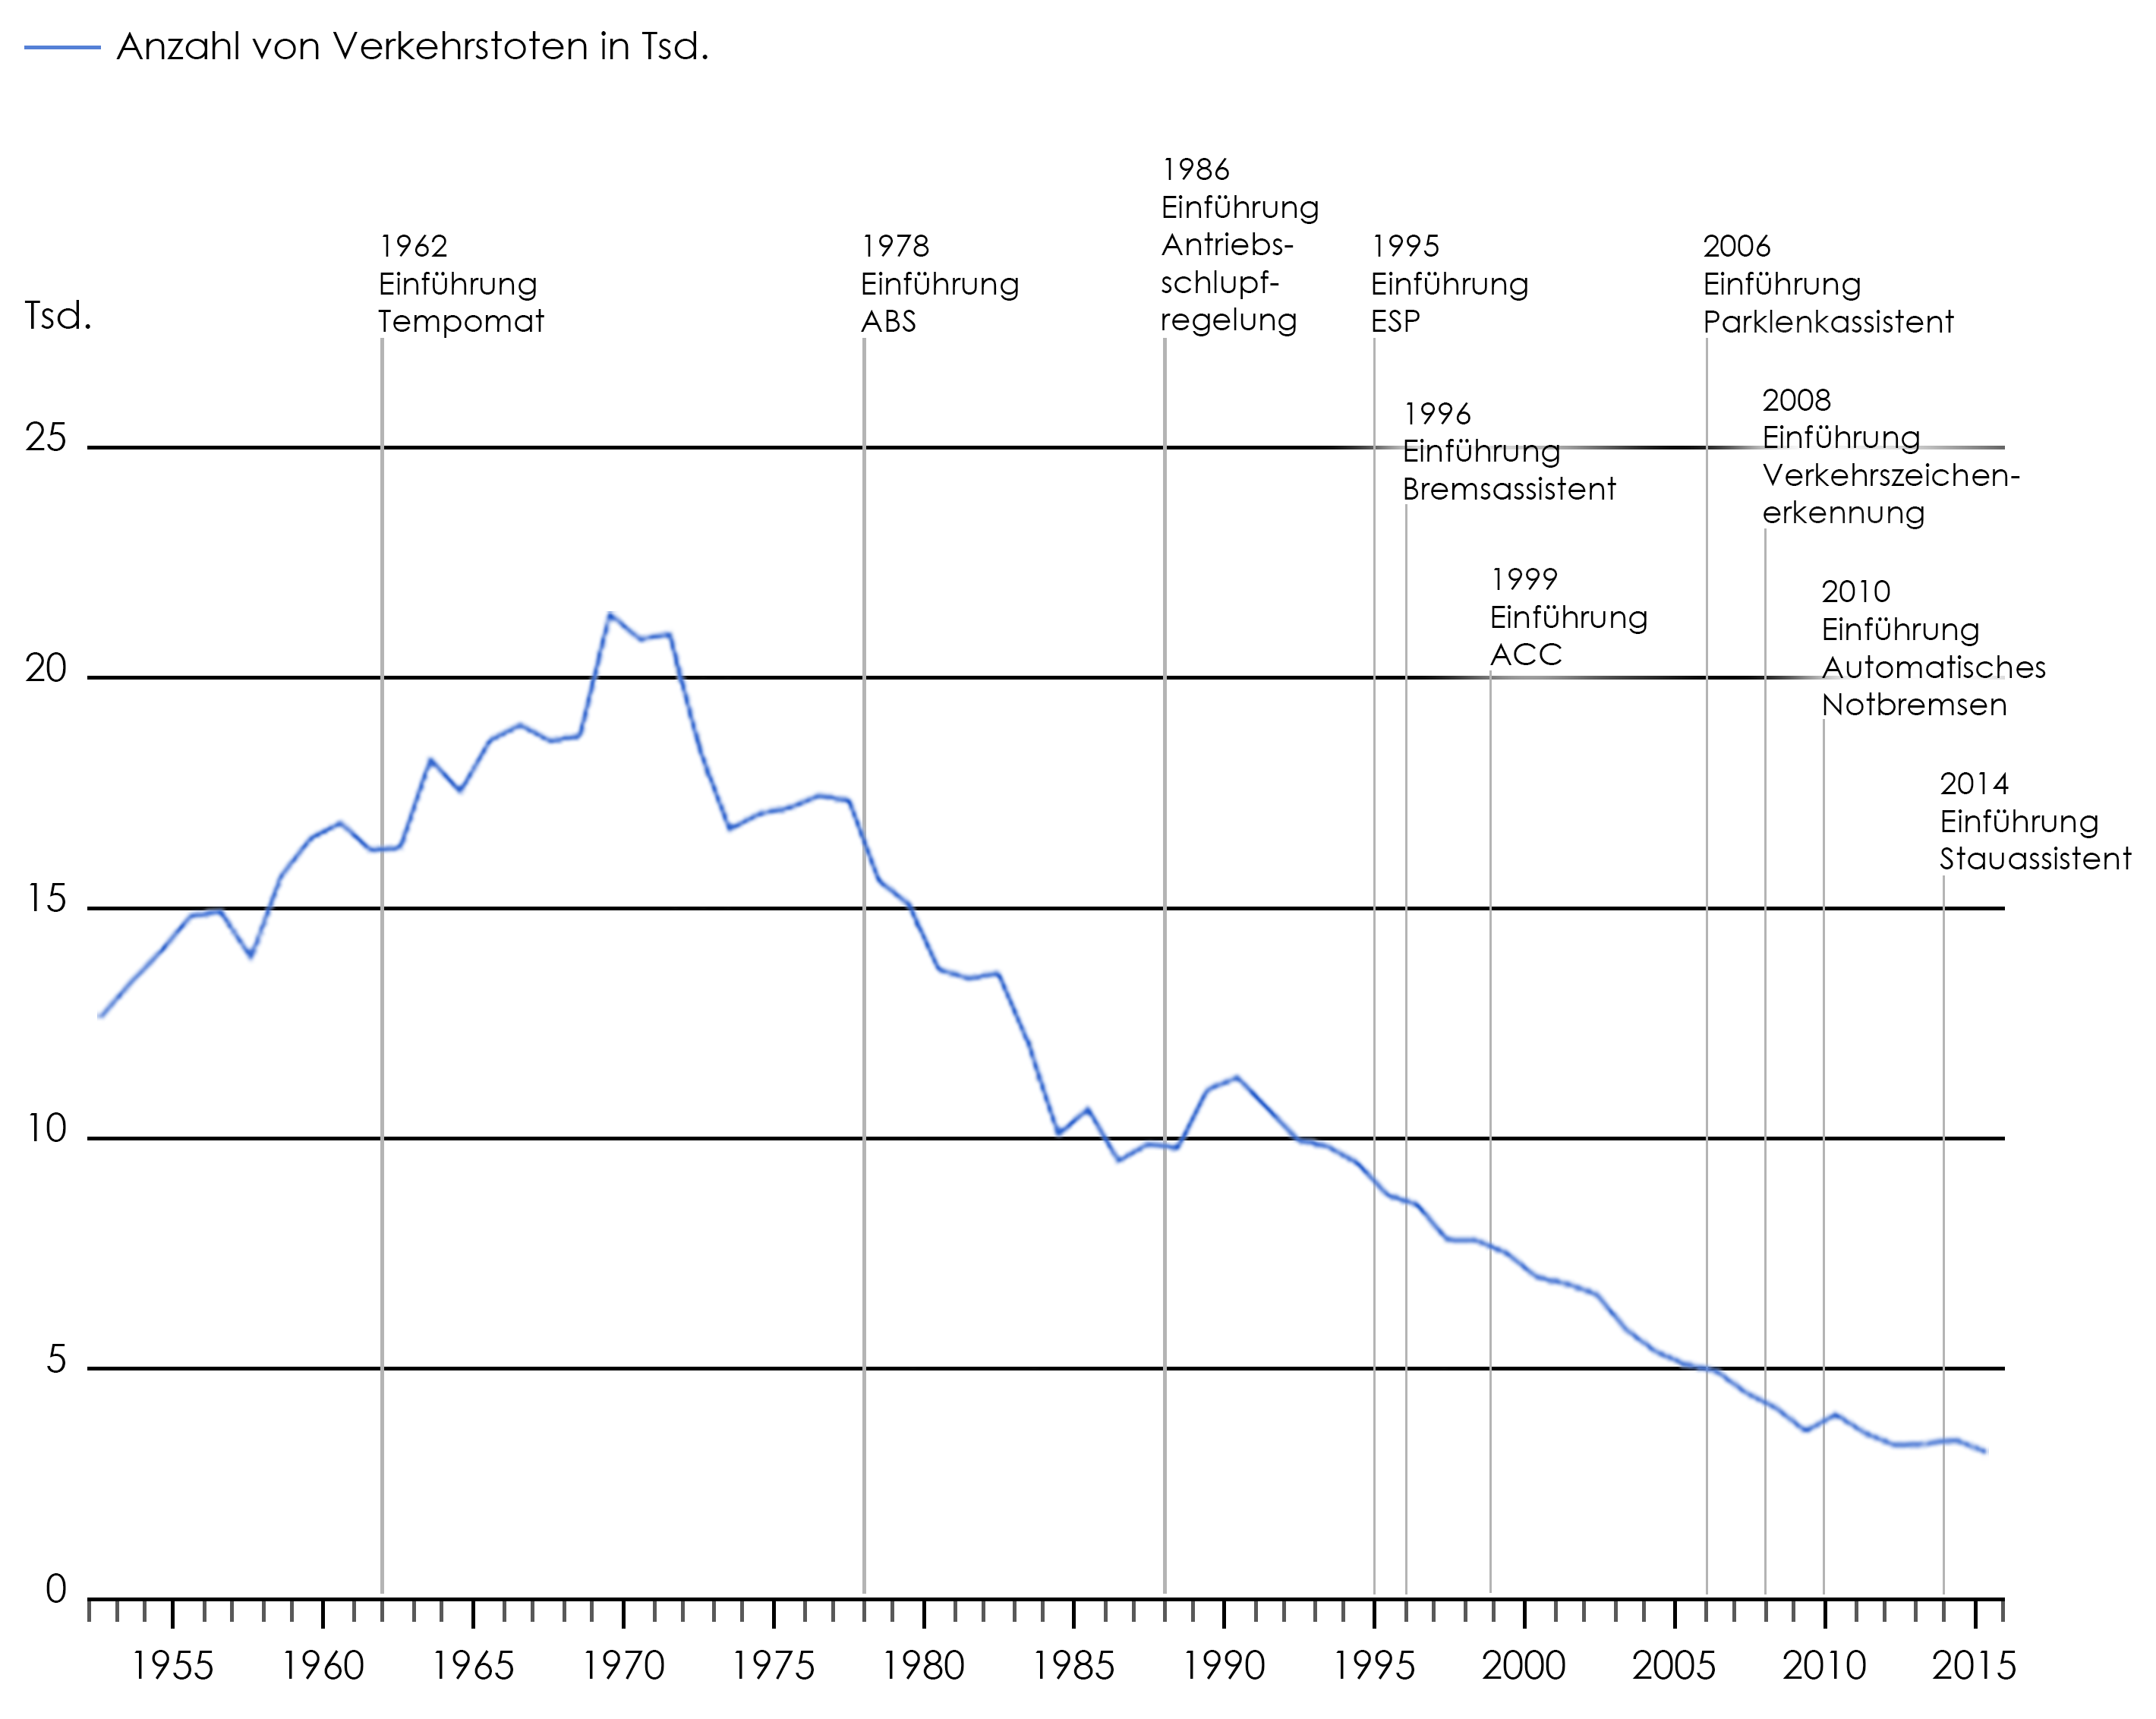
\includegraphics[width= 0.95\textwidth]{images/statistik1}
	\caption[Verlauf der Anzahl an Todesopfer im deutschen Straßenverkehr von 1953 bis 2016 in Kombination mit Einführung von Fahrerassistenzsystemen]{Statistik der Todesfälle im deutschen Straßenverkehr mit Einführungsdaten von FAS; Quelle: Statistisches Bundesamt \protect\cite{sba}}  
	\label{fig:sba}
\end{figure}

\subsection{Zielsetzung}
\glqq Die Automatisierung der Fahrzeugführung verändert die Anforderungen an das kognitive System des Autofahrers grundlegend. Um daraus keine Gefahren entstehen zu lassen, sind noch zahlreiche Fragen offen.\grqq{} \cite{schlott}. Schlott trifft diese Aussage um die kritischen Aspekte der hochautomatisierten Fahrt zu beleuchten und um auf mögliche Risiken hinzuweisen. 

Diese Arbeit befasst sich sowohl mit der Erhebung der technischen Grundlagen, als auch mit dem menschlichen Informationsverarbeitungsprozess. Die Erkenntnisse aus den einzelnen Bereichen werden aggregiert und miteinander verknüpft, um somit die Basis für ein umfassendes HMI-Konzept zu generieren. Dieses soll die benötigten Informationen aller Automatisierungsstufen zur Förderung des Vertrauens in das Gesamtsystem und Aufrechterhaltung des Situationsbewussteins darstellt, um den Fahrer zu unterstützen. 

Das auszuarbeitende Konzept soll in einem Entwicklungsfahrzeug, weitere Details siehe \autoref{sec:entfahr}, eingesetzt werden und umfasst somit nur die Automatisierungsstufen 0 bis 3, da zum aktuellen Zeitpunkt noch keine aktiven Fahrerassistenzsysteme für höhere Automatisierungsstufen zur Verfügung stehen. Dazu wird folgende Forschungsfrage gestellt: \\

\begin{tabular}{p{0.3cm} p{0.5cm} p{13cm} p{0.5cm}}
	& \textbf{RQ}	& Können die bla bla? & \\
\end{tabular}
\vspace{1em} 

Es wird angenommen, dass sich das Informationsbedürfnis des Fahrers über die Automatisierungsstufen unterschiedlich verhält und eine sich dynamisch veränderbare Anzeige gefordert wird. Daraus lassen sich folgende Hypothesen ableiten: \\

\begin{longtable}{p{0.3cm} p{0.5cm} p{13cm} p{0.5cm}}
	& \textbf{H1}	& Je höher, desto geringer. & \\
	& & & \\
	& \textbf{H2}	& Bla bla, bla bla. & \\
	& & & \\
	& \textbf{H3}	& Bla bla, bla bla. & \\
\end{longtable}